%!TEX root = thesis.tex

%%%%%%%%%%%%%%%%%%%%%%%%%%%%%%%%
% intro.tex: Introduction to the thesis
%%%%%%%%%%%%%%%%%%%%%%%%%%%%%%%%
\chapter{Introduction}
\label{chap:intro}


A galaxy's morphology is the culmination of its formation, interactions, and evolution through environmental and internal processes. It is a snapshot into the current state of a galaxy's life as well as window to its past. The insights gleaned through the study of galaxy morphology have radically changed our view of universe since the time of Edwin Hubble. 


Astronomers have made use of visual galaxy morphologies to understand the dynamical structure of these systems for nearly ninety years 
\citep[e.g.,][]{Hubble1936, 
			deVauc1959, 
			Sandage1961, 
			vandenBergh1976, 
			NairAbraham2010, 
			Baillard2011}. 
The division between early-type and late-type systems corresponds, for example, to a wide range of parameters from mass and luminosity, to environment, color, and star formation history 
\citep[e.g.,][]{Kormendy1977,  
			Dressler1980, 
			Strateva2001, 
			Blanton2003a, 
			Kauffman2003, 
			Nakamura2003, 
			Shen2003, 
			Peng2010}; 
while detailed observations of morphological features such as bars and bulges provide information about the history of their host systems 
\citep[e.g.,][]{KK04, 
			Elmegreen2008, 
			Sheth2008, 
			Masters2010, 
			Simmons2014}. 
Modern studies of morphology  divide systems into broad classes 
\citep[e.g.,][]{Conselice2006, 
			Lintott2008, 
			Kartaltepe2015, 
			Peth2016}, 
but a wealth of information can be gained from identifying new and often rare classes, such as low redshift clumpy galaxies \citep[e.g.,][]{Elmegreen2013}, polar-ring galaxies \citep[e.g.,][]{Whitmore1990}, and the green peas \citep{Cardamone2009}. 

Obtaining these morphologies has traditionally been a time-consuming visual endeavor and only in the past twenty years have automated morphological assignment been possible. Even with the varied automated approaches currently being exploited, an era of Even Bigger Data looms for the field of astronomy. The next decade will herald the first light of more powerful ground- and spaced-based telescopes such as the Large Synaptic Survey Telescope (LSST), Euclid, and WFIRST. The surveys planned for these instruments promise to revolutionize the field of astrophysics providing several orders of magnitude more data than is currently available. Traditional techniques will not be sufficient for extracting galaxy morpholgoies on a pertinent timescale. 

This thesis details a solution to the scalability of galaxy morphology designations by examining classifications obtained as part of the Galaxy Zoo project, a crowd-sourcing initiative that has obtained morphological classifications from thousands of volunteers for over a million galaxies from several astrophysical surveys. Though innovative, even crowd-sourcing will be unable to sustain the classification load for future surveys. Instead, these classifications are combined with supervised machine learning algorithms that train on automated measurements of galactic morphological structural indicators. This thesis begins with a detailed account of the data utilized in this work as well as the methodology used to obtain these morphology diagnostics (Chapter \ref{chap:2}). Chapter \ref{chap:3} demonstrates how crowd-sourcing techniques can be optimized by applying a Bayesian approach to aggregation of Galaxy Zoo classifications, while Chapter \ref{chap:4} explores the combination of these visual classifications with machine learning algorithms. Also included is a prelimary analysis of a rare sample of ``clumpy'' galaxies in the local universe discovered during the course of the analysis of Galaxy Zoo classifications (Chapter \ref{chap:5}). While common in the distant universe, these potential local counterparts could shed light on star formation as it pertains to the formation of galactic bulges. This Introduction provides a brief overview of galaxy formation, the sciece achieved through the study of morphology, and galaxy classification techniques, as well as an overview of Galaxy Zoo: Express (GZX), an integrated framework of human and machine galaxy classifiers. 


%%%-------------------------------------------------------
%%% SECTION:    GALAXY FORMATION
%%%-------------------------------------------------------
\section{Galaxy formation}
According to the $\Lambda$CDM model, the first galaxies are theorized to have formed from primordial density fluctuations shortly after the Big Bang. These fluctuations are charactized as local overdensities. These regions experience gravitational instability which causes them to grow with time according to a power law. When the overdensity is in the linear regime ($\delta\rho/\rho <<1$) the size of the regions expand with the expansion of the universe. As they continue to grow they eventually reach a turning point ($\delta\rho/\rho\sim1$), break away from the expansion, and start to collapse, eventually forming self-gravitating structures. 

These collapsing structures contain both baryonic and dark matter. The latter relaxes violently to create a dark matter halo, while the baryonic matter shocks to the virial temperature. In order for stars to form this gas must cool, and various mechanisms are possible depending on the temperature: bremsstrahlung emission in the hottest regimes, and various methods of excitation and de-excitation in cooler regimes. As the gas cools it collapses further and likely fragments into small, highly dense cores that eventually form the first stars. 

Population III stars were formed entirely of primordial gas consisting solely of hydrogen and helium, as heavier elements were not yet synthesized. These stars were likely the most massive stars ever created and thus had short life spans before dying brilliantly in the first supernovae. As these stars formed at $z\sim11$ no confirmed observations have been recorded and thus the details are obscure. However it is well established that their demise distributed the first heavier elements from which subsequent stars formed. Today, Population I stars are the most metal-rich. 

If the collapse of the gas in the dark matter halo retained angluar momentum it would be conserved through the formation of a disk. However, the disks of galaxies in the distant universe may not be like those of today as discussed later in this chapter. Feedback processes such as the blast waves and energy released during supernovae, and the active accretion of supermassive black holes known as active galactic nuclei (AGN) can affect the course of a galaxy's development. 

The current paradigm also supports that these systems grow hierarchically in that larger dark matter halos are built from the coalescence of smaller systems. If these halos contain galaxies, those too can merge which results in identifiably distinct morphologies as will be discussed below. 




%%%-------------------------------------------------------
%%% SECTION:    STANDARD MORPHOLOGY DESIGNATIONS
%%%-------------------------------------------------------
\section{Standard morphology designations}


%%%-------------------------------------------------------
%%% FIGURE:    HUBBLE TUNING FORK
%%%-------------------------------------------------------
\begin{figure}
\centering
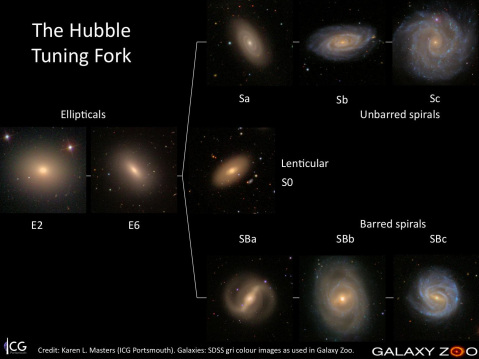
\includegraphics[width=5in]{Figures/Masters_tuningfork.jpg}
\caption[Hubble tuning fork]{The Hubble ``tuning fork'' with example images for each galaxy type created from $gri$-composite SDSS imaging. Credit: Karen L. Masters and the Sloan Digital Sky Survey (SDSS) Collaboration.}
\label{fig: tuning fork}
\end{figure}

The oldest and arguably simplest system for categorizing galaxy morphology dates back to the 1930s and Edwin Hubble's famous ``tuning fork'' \citep{Hubble1926, Hubble1936}. Based on a small sample, Hubble classified galaxies into two major groups, elliptical and spiral. Visually, elliptical galaxies possess a smooth light distribution, while spirals are characterized by a well-defined disk structure often with spiral arms. Hubble assigned a number to elliptical galaxies denoting the degree of their ellipticity, where 0 corresponds to a nearly perfectly round galaxy and 7 being highly elongated. Spirals were given additional designation in the form of letters `a' through `c', characterizing the compactness of their spiral arms. For example, ``Sa'' galaxies are tightly wound, whereas ``Sc'' spirals are looser. The spiral category was then further subdivided by galaxies that exhibited a central bar. There are also indications that the bulges inherent to many spiral galaxies share a close connection to elliptical galaxies, thus the transitional ``S0'' category: galaxies with disks that are dominated by the bulge component. 

It became common to call galaxies on the left side of the diagram ``early-types,'' and those on the right ``late-types''. Contrary to this author's belief, Hubble never intended these designations to imply galactic evolution. Instead, this terminology was borrowed from stars, where massive O and B stars were referred to as ``early-type,'' while older stars were known as ``late-type''\citep{Buta2011}. It has subsequently become clear that, much to the contrary, ellipticals are dominated by late-type stars, while disk galaxies are typically composed of young, early-type stars.  Unfortunately, the misnomer has stuck. 


This method of galaxy classification was based on an extremely small sample of which only a few percent did not conform to the basic designations originally posited by Hubble. These leftover galaxies were dubbed ``irregulars'' or ``peculiars''. It wasn't until much later that it was discovered this galaxy type was far more prevalant than Hubble originally thought, especially in the more distant universe. Since this early attempt at classification, several other systems have been put forward but most share the same basic categories \citep[e.g.,][]{deVaucouleurs1959, Conselice2006}. Indeed, even this simplistic approach has yielded nearly a hundred years of science that has advanced our understanding of galaxy formation, structure, and evolution. 
 

%%%-------------------------------------------------------
%%% SECTION: MORPHOLOGY AS A TRACER OF GALAXY EVOLUTION
%%%-------------------------------------------------------
\section{Morphology as a tracer of galaxy evolution}
That galaxies exhibit different features is obvious, but what, if anything, do those features tell us? Because we cannot observe the entire lifespan of a single galaxy it is fair to question whether or not morphology is primarily an indicator of age, with galaxies marching starkly through the Hubble sequence, or whether dynamical processes shape that morphology. Or both. In this section we discuss some of the major roles that galaxy morphology has played in understanding the evolution and formation of these systems. 


 %Galaxy morphology is strongly correlated with galactic star formation history. Galaxies where star formation ceased gigayears ago tend to look very different from those where star formation continues at the present time. 

%%%-------------------------------------------------------
%%% SECTION:       STELLAR POPULATIONS 
%%%-------------------------------------------------------
\subsection{Stellar populations and star-formation histories}
At its heart, morphology simply traces an integrated 2D projection of a galaxy's light distribution. As such, it encodes information on the distribution of a galaxy's stellar, gas, and dust content. However, these components are best traced through different wavelengths of light. 

Consider a coevolving stellar population with a mass distribution according to your favorite initial mass function. Stars on the Main Sequence (MS) radiate in the blue and ultraviolet (UV) end of the spectrum due to their high effective temperatures. The most massive quickly evolve off the MS and become red supergiants causing a decrease in the UV flux and an increase in the near infrared (NIR). As the low mass stars in this stellar population continue to evolve off the MS, the UV flux steadily decreases until eventually the red giant branch becomes the dominant source of flux, radiating in the IR. This so-called \textit{passive} evolution indicates that as a galaxy ages it becomes redder. A galaxy's morphology is tightly correlated with its color: massive elliptical galaxies are typically referred to as ``red and dead,'' possessing old stellar populations, while disk galaxies are generally still undergoing star formation and thus possess young, bluer stellar populations \citep[e.g.,][]{Strateva2001,Baldry2004b, Cirasuolo2007, Lee2013, Taylor2015}. This dichotomy is so prevalent that color has been used as a proxy for morphology when acquiring the latter was impractical \citep[e.g.,][]{Shen2003, Blanton2003c}. 

Furthermore, this color bimodality correlates with luminosity resulting in the color-magnitude relation (CMR) \citep{Baldry2004a, Bell2004}. Now ubiquitous, this relation visualizes the separation of galaxy colors as a function of luminosity resulting in three main categories: the blue cloud, the red sequence and, more recently recognized, the green valley. Studies have shown that the red sequence is dominated by early-type galaxies like elliptical/S0, while disk galaxies reside in the blue cloud. There is a distinct gap between these two galaxy populations but recent studies have shown that, though sparse, galaxies residing in this region could be in the middle of active evolution sparking morphological change \citep{Schawinski2007}. The top panel of Figure \ref{fig: CMR} shows an example of the color-magnitude relation for a sample of SDSS galaxies, while the bottom panel depicts a schematic of the associated morphologies \citep{Kormendy2012}. 

%%%-------------------------------------------------------
%%% FIGURE:   COLOR MAGNITUDE RELATION
%%%-------------------------------------------------------
\begin{figure}
\centering
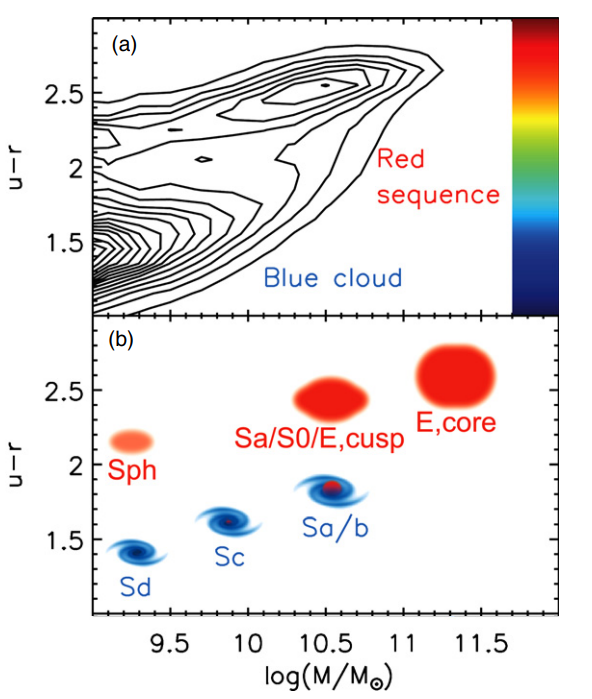
\includegraphics[width=3.5in]{Figures/kormendy_CMR.png}
\caption[Galaxy color-magnitude relation.]{Color-magnitude relation adapted from \cite{Kormendy2012}. Though the x-axis is in units of log stellar mass, mass correlates strongly with a galaxy's luminosity. The top panel shows the contours of galaxy number density \citep{Baldry2004b} with the rainbow bar denoting the associated $u-r$ color. The botton panel depicts the dominant galaxy morphologies associated with each location.}
\label{fig: CMR}
\end{figure}

The color-magnitude relation is tighter for early-type galaxies providing a tool to constrain the star-formation histories of this galaxy population \citep{Sandage1978, Tully1982}. There exists a degeneracy between the age and metallicity of stellar populations: though older stars tend to be redder, this effect can also be achieved through an increase in stellar metallicity. It is now believed that the slope of the CMR is due primarily to metallitcy effects \citep{Bower1992, Kodama1997}, which then allows for age estimates to be placed on the last episode of significant star formation in early-type galaxies \citep[e.g.,][]{LopezCruz2004}. The small scatter in this relation reflects that these galaxies have old, passively evolving stellar populations. 

put this somewhere \citep{Mei2009}
%Galaxies contain more than just stars; gas and dust can also alter a galaxy's morphology. Dust is thought to be produced in AGB stars and distributed to the interstellar medium via stellar winds. Disk galaxies typically have more dust than ellipticals indicating that early-type galaxies expelled their dust content via dramatic mergers \citep{some people}. Blue light is more strongly attenuated than red light. This causes the dust to heat and radiate in the IR making a galaxy appear redder than it would otherwise. Another, more dramatic example of dust's effect on a galaxy's morphology is the dust lanes exhibited by many spiral galaxies. 

%It is clear that to fully understand a galaxy's composition, studying the morphology through observations across the electromagnitic spectrum is necessary: cold dust indicative of recent galaxy-galaxy interaction can be determine through radio observations of HI gas; infrared observations shed light on the dust content and old stellar components, visual and UV observations trace ever stellar nurseries, and high energy observations like X-rays give a tantalizing peak at what lurks in the bulges of active galaxies. 

%%%-------------------------------------------------------
%%% SECTION:  MASS ASSEMBLY
%%%-------------------------------------------------------
\subsection{Mass assembly and the emergence of the Hubble sequence}
The most fundamental characteristic of a galaxy is its mass. Though not as easy to measure as luminosity, it is now believed that several processes within a galaxy are directly tied to stellar mass. Stellar mass functions (SMFs) are thus a key first-order observable that statistically traces the formation of stars in the universe. Another key property is a galaxy's star formation rate (SFR).  A cottage industry for decades, constructing mass and star-formation density functions has provided insights into the build-up of baryonic mass over cosmic time. 

Understanding the rate of growth and distribution of baryonic mass in galaxies provides constraints on the mechanisms necessary to produce such observations. It is well known that star formation density of the universe increased from the earliest epochs up until $z\sim2$ and has substantially declinced since then, as shown in the Lilly-Madau plot in Figure \ref{fig: SFR density} \citep[and references therein]{Madau2014}.  However this rapid build up of stellar mass was not distributed equally among all galaxies. Furthermore, the subsequent evolution of these systems provide clues to the emergence of the galaxy morphologies we see today. 

\begin{figure}
\centering
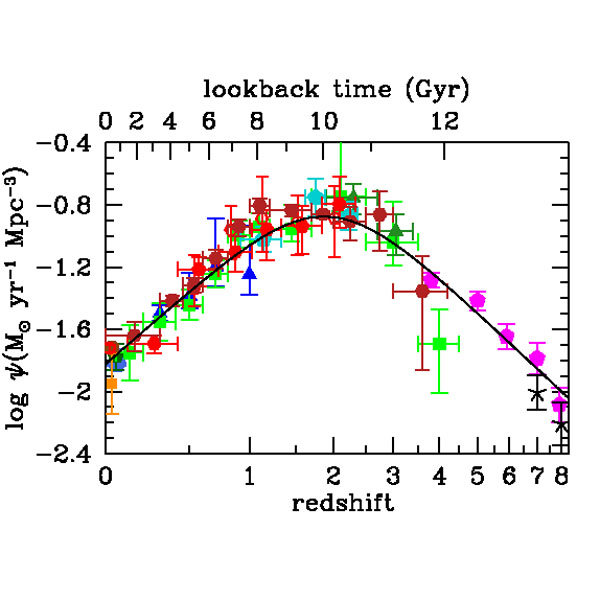
\includegraphics[width=5in]{Figures/MadauDickinson2014.jpg}
\caption[The history of cosmic star formation.]{The history of cosmic star formation as determined by FUV+IR rest-frame measurements from several galaxy samples \citep[credit:][and references therein]{Madau2014}. This shows that cosmic star formation experienced peaks around $z\sim2$ when the universe was approximately 3.5Gyr old followed by a gradual decline until present day.}
\label{fig: SFR density}
\end{figure}

At $z>2$, most of the stellar mass density resides in irregular galaxies, and the existence of disk galaxies is questionable \citep{Dickinson2000,Papovich2005,Cameron2011,Conselice2005,Conselice2011,Buitrago2013}. However, mass functions constructed according to morphological type as a function of redshift show that the stellar mass density gradually begins to reside more in disk systems at $1<z<2$, and in the local universe, is dominated by early-type galaxies though statistics differ \citep{Brinchmann2000, Bell2003, Bundy2005, Mortlock2013, Kelvin2014, HuertasCompany2016, Thanjavur2016}. Thus considerable evolution has occured such that high-redshift systems settle down into the galaxies we see in the local universe.

Heirarchical galaxy formation theory predicts the build up of smaller systems before the creation of larger galaxies by way of violent mergers, simultaneously transforming disk morphologies into spheroidal systems \citep{Driver2013,Bluck2009,Man2012}, Indeed, this is likely the case in the high-redshift universe, but after $z<2$, the dominant mechanism for galaxy evolution switches to cold gas accretion and with it, the formation of disk galaxies from irregular systems \citep{Conselice2013}. Both mergers and gas accretion processes are observed to be mass-dependent with the most massive galaxies settling into the familiar Hubble sequence more quickly than low-mass galaxies \citep{Buitrago2013,Conselice2011,Mortlock2013}. This so-called ``downsizing'' process, though seemingly contradictory to the heirarchical theory, is nevertheless favored observationally \citep{Cowie1996, Brinchmann2000, Bundy2005}. 

%%%-------------------------------------------------------
%%% SECTION:   MORPHOLOGY AND ENVIRONMENT
%%%-------------------------------------------------------
\subsection{Morphology as a function of environment}
A galaxy's environment also has a direct relationship with its morphology. First quantified by \cite{Dressler1980}, the morphology-density relation is an emperical observation that elliptical galaxies tend to reside in the densest environments, i.e., rich groups and clusters, at all stages of cosmic time. in the richest and densest clusters of galaxies, the dominant morphology is elliptical, while for field galaxies, the dominant morphology is spiral. Furthermore, it's been determined that this relation evolves over time, at least for the densest environments. All of this points to scenarios in which the environment of a galaxy influences its morphology \citep[e.g.,][]{Fasano2000, Shen2003, Smith2005, Peng2010}

Much study has been done to separate the effects of environment from mass, i.e., secular, causes of morphological features. Peng, Shen,,etc. Cluster environments are, compared to the field, extremely hot and dense. Galaxies residing in these environments have faster velocity dispersion, on average.   It's estimated that field galaxies are, on average, 1 per Mpc (?). The merging rate depends on the density of galaxies. In the past galaxies were closer together so merging was a bigger deal. Logically then, it would seem that merging happens all the time in clusters and that this subsequently causes a morphological change from disk to elliptical. However, galaxies are moving so briskly in clusters that it becomes less likely that they collide! Instead, mergers seems to be a predominant morphological mechanism in groups rather than clusters. In clusters, instead, other physical processes shape the way a galaxy evolves and looks over time. 

Spirals convert to S0/elliptical galaxies in clusters due to several processes: they should have lost their cold atomic and molecular gas via ram pressure stripping (but see Tonnesen \& Bryan 2009, for the effect of ram
pressure on molecular clouds), harassment (Moore et al. 1996),
strangulation (Kawata \& Mulchaey 2008), etc.


%mergers and AGN \citep{Kocevski2012, Villforth2014}

%%%-------------------------------------------------------
%%% SECTION:    RARE MORPHOLOGIES
%%%-------------------------------------------------------
\subsection{Insights from rare morophologies}
While great insight into the formation and evolution of galaxies has been gleaned through examination of broad morphological categories, more can be learned by digging into the details. Any theory of galaxy evolution will have to account for the dizzying array of galactic forms including the development of bars, bulges, and rings, as well as rare morphologies such as the ``green peas,'' or giant clumps of star formation in galaxies in the nearby universe.

Identifying finer details of galactic structure has become easier with the the advent of cameras aboard the Hubble Space Telescope. Features like bars and bulges directly relate to a galaxy's history. However, it has only been since the development of large scale surveys like SDSS, CANDELS, DeCALS(?) that astronomers have become aware of rare populations of galaxies. While small, these populations provide a means to constrain formation and evolution theories. 

First recognized as an individual class of galaxies by Galaxy Zoo volunteers in 2007, the ``green peas'' are a type of luminous blue compact galaxy whose name reflects the hue of these galaxies in the false color SDSS images presented during the Galaxy Zoo project. These oxygen-rich objects are observed to have some of the largest star formation rates with some of the smallest masses. It is surmised that these galaxies were commonplace in the early universe and likely played a large role in the reionization of the universe. That such galaxies exist in the local universe provides a way to probe the cosmic past. 

Another class of potential local analogs of high-redshift counterparts are low redshift ``clumpy'' galaxies. As previously discussed, galaxies of the past were largely irregular with star formation rates much higher than today. Much of the peculiar shapes of these galaxies are due to massive knots of star formation. These galaxies underwent processes that transformed them into disk galaxies with the result being that this particular morphology is rather rare in the local universe. These star-forming clumps are though to form via gravitational disk instability \citep{Toomre???}. If these features are long-lived compared to their host galaxy, it is possible they contribute to the growth of the galactic bulge. Chapter 5 presents a more in depth discussion and preliminary analysis of a sample of such galaxies discovered through the Galaxy Zoo project.


\section{Obtaining morphologies}
A galaxy's morphology is thus an integral component for understanding the nature of these systems as well as their formation and evolution in the fullest sense. Obtaining such morphological information poses several challenges. This section will discuss the methods in which galaxy morphologies are collected and quantified. 

\subsection{Visual classifications}
For most of the past century, galaxy morphologies were determined by a small number of expert astronomers beginning with Hubble. Visual classification, though highly accurate due to the human mind's unique pattern recognition capability, is, however, entirely slow. For decades assignment of morphological type to galaxies resulted in small samples with varying degrees of label complexity and often lacking in statistical significance \citep{Hubble1936, Sandage1961, SandageTammann1981, deVaucouleurs1963, deVaucouleurs1991}. With surveys like the Sloan Digital Sky Survey \citep[SDSS,][]{Abazajian2003} and the CFHTLS-Deep Survey, coupled with cartels of graduate student classifiers, samples approached the tens of thousands \citep{Fukugita2007, Schawinski2007, NairAbraham2010}.

Unfortunately, this approach still cannot take full advantage of the depth and scope of such large scale surveys. This necessitated the birth of the Galaxy Zoo (GZ) project \citep{Lintott2008, Lintott2011, Willett2013, Willett2017, Simmons2017}, the first effort to crowd-source the task of galaxy morphology to the general public. With thousands of citizen scientists classifying, GZ has released visual morphologies for over one million galaxies providing a solution that scales visual classification for current surveys and producing a prolific amount of scientific output \citep[e.g.,][]{Land2008, Bamford2009, Darg2010, Schawinski2014, Galloway2015, Smethurst2016}.
A hybrid approach is the system developed by the Cosmic Assembly Near-infrared Dark Energy Legacy Survey \citep[CANDELS;][]{Grogin2011, Koekemoer2011} team, imaging produced by the Hubble Space Telescope. This scheme \citep{Kartaltepe2015} crowd-sources not to the general public, but to dozens of expert astronomers collecting visual classifications for over 50,000 galaxies in the CANDELS fields. 
%upcoming surveys such as \textit{LSST} and \textit{Euclid} will require a different approach, imaging more than a billion new galaxies  \citep{LSST, Euclid}.  If detailed morphologies can be extracted for just  0.1\% of this imaging, we will have millions of images to contend with. A project of this magnitude would take more than sixty years to classify at Galaxy Zoo's current rate and configuration. Standard visual morphology methods will thus be unable to cope with the scale of data. 


\subsection{Automated classifications}
Another approach has been the automated extraction of morphologies with the development of parametric \citep{Sersic1968, Odewahn2002, Peng2002}, and non-parametric 
\citep{Abraham1994, 
	   Conselice2003, 
	   Abraham2003, 
	   Lotz2004,  
	   Freeman2013} 
structural indicators. While these scale well to large samples 
\citep[e.g.,][]{Simard2011, 
			Griffith2012, 
			Casteels2014, 
			Holwerda2014, 
			Meert2016}, 
they often fail to capture detailed structure and can provide only statistical morphologies with large uncertainties \cite[e.g.,][]{Abraham1996, Bershady2000}. We briefly highlight a few of these indicators here while a more detailed discussion can be found in Chapter 2. 

One of the first and most popular parametric approaches for modelling a galaxy's light distribution is the S\'ersic profile:
\begin{equation}
I(R) = I_e \exp \Big(-b_n\Big[\Big(\frac{R}{R_e}\Big)^{1/n}-1\Big]\Big)
\end{equation}
where $I_e$ is the intensity at the ``effective'' radius $R_e$ that encloses half of the total light from the model, $n$ is the S\'ersic index that essentially describes the concentration of the light profile, and $b_n$ is a term that depends on $n$. When $n=4$, produces the de Vaucouleurs law which well describes the light profile of elliptical galaxies. On the other hand, a Sersic index of $n=1$ reduces the equation to an exponential which is a good description for disk galaxies. This index has been used for decades as a broad method to classify galaxies into early- and late-type categories. 

A drawback to the parametric approach is the need to assume the underlying distribution and while this works technique works well for galaxies that are obviously elliptical or spiral, it produces mixed results for other morphological types, i.e., irregulars or peculiars, which have low central concentration resulting in a low Sersic index, but which do not have disks or spiral arms. Additionally, fitting this function to thousands or even millions of galaxies is time consuming. Non-paramteric structural indicators require fewer assumptions and are derived empirically.

Closely related to the Sersic index is the non-paramatric diagnostic of concentration. Originally conceived by \cite{Abraham1996}, it has several definitions but each measures the ratio of the aggregated light within two concentric apertures about the galaxy's center: one close to the galaxy's center and the other further out. Typically, these apertures contain 50 and 90\% of the galaxy's total light. Measuring a galaxy's concentration can be much faster than fitting it with a Sersic profile and less prone to fitting failures. 

Once these parametric and non-parametric diagnostics have been computed for a sample of galaxies it is then common practice to place a cut on one or more of these parameters to separate the sample into early- and late-types \citep{Shen2003}. More sophisticated approaches involve measuring several automated diagnostics and separating galaxies in a two dimensional plane, a technique that has been highly successful at identifying not only distinctions between spheroidal and disk-like galaxies but also merging and interacting galaxies \citep{Lotz2004, Lotz2006,Conselice2000, Conselice2003,Freeman2013}. 


 %Several of these diagnostics have been developed over the past couple decades, each probing a different part of the galaxy's light profile and thus its overall dynamical distribution. The most common diagnostics are described in greater detail in Chapter 2. 
%Example of using parametric Sersic profile to classify galaxies as early-/late-type: ``We show that the wavelength-dependence of n may be employed to separate visually-classified early- and late-type galaxies in a manner similar to the use of colour and n. Furthermore, we find that the wavelength variation of n can recover galaxies that are misclassified by these other morphological proxies."\citep{Vika2015}





\subsection{Machine learning}
Machine learning techniques are becoming increasingly popular for classification and image processing tasks. Another automated approach, these generally work by defining a set of features that describe the morphology in an $N$-dimensional space. These features can be anything: color, mass, spectral index, velocity dispersion, and of course the parametric and non-parametric indicators discussed above. Choosing which features are most appropriate will depend on the classification task at hand, the particular machine learning algorithm choosen, and the strength of the correlation between a given feature and the galaxy's intended class. 

The location in this $N$-dimensional morphology space defines a morphological type for each galaxy. Learning the morphology space can be achieved through algorithms such as Support Vector Machines \citep{HuertasCompany2008} or Principal Component Analysis \citep{Watanabe1985, Conselice2006, Scarlata2007, Peth2016}. Another approach is through deep learning, a machine learning technique that attempts to model high level abstractions. Algorithms like convolutional and artificial neural networks (CNNs, ANNs) have been used for galaxy morphology classification with impressive accuracy \citep{Ball2004, 	Banerji2010, Dieleman2015, HuertasCompany2015}. 

A drawback to all machine learning classification techniques is the need for standardized training data, with more complex algorithms requiring more data. Furthermore, these data are best when consistent for each survey: differences in resolution and depth can be implicitly learned by the algorithm making their application to disparate surveys challenging. 


\section{Overview of Galaxy Zoo: Express}

 In this work we present a system that preserves the best features of both visual and automatic classifications, developing for the first time a framework that brings both human and machine intelligence to the task of galaxy morphology to handle the scale and scope of next generation data. We demonstrate the effectiveness of such a system through a re-analysis of visual galaxy morphology classifications collected during the Galaxy Zoo 2 project, and combine these with a Random Forest machine learning algorithm that trains on a suite of non-parametric morphology indicators widely used for automated morphologies. In this paper we focus on the first question of the Galaxy Zoo decision tree. We demonstrate that our method provides a factor of 11.4 increase in the rate of galaxy morphology classification  while maintaining at least 93.5\% classification accuracy as compared to Galaxy Zoo 2 published data. We first present an overview of our framework, which also serves as a blueprint for this paper. 


%%%-------------------------------------------------------
%%% FIGURE:     GZ EXPRESS Schematic
%%%-------------------------------------------------------
\begin{figure*}[ht!]
%\figurenum{1}
\plotone{Figures/human_machine/f1.pdf}
\caption[Schematic of the Galaxy Zoo: Express human+machine hybrid system.]{Schematic of our hybrid system. Humans provide classifications of galaxy images via a web interface. We simulate this with the Galaxy Zoo 2 classification data described in Chapter~\ref{chap:2}. Human classifications are processed with an algorithm described in Chapter~\ref{chap:3}. Subjects that pass a set of thresholds are considered human-retired (fully classified) and provide the training sample for the machine classifier as described in Chapter \ref{chap:4}. The trained machine is applied to all subjects not yet retired. Those that pass an analogous set of machine-specific thresholds are considered machine-retired. The rest remain in the system to be classified by either human or machine. This procedure is repeated  nightly. \label{fig: schematic}}
\end{figure*}


%%----------------------------------------------------------------------------------------------------------------------------------------------------
%%   GALAXY ZOO EXPRESS OVERVIEW
%%---------------------------------------------------------------------------------------------------------------------------------------------------

The Galaxy Zoo Express (GZX) framework combines human and machine to increase morphological classification efficiency, both in terms of the classification rate and required human effort. Figure~\ref{fig: schematic} presents a schematic of GZX including section numbers as a shortcut for the reader. We note that transparent portions  of the schematic represent areas of future work which we explore in Chapter \ref{chap:summary}. Any system combining human and machine classifications will have a set of generic features: a group of human classifiers, at least one machine classifier, and a decision engine which determines how these classifications should be combined.

In this work we demonstrate our system through a re-analysis of  Galaxy Zoo 2 (GZ2) classifications. This allows us to  create simulations of human classifiers. These classifications are used most effectively when processed with SWAP, a Bayesian code described in Chapter \ref{chap:3}, first developed for the Space Warps gravitational lens discovery project~\citep{Marshall2016}. These subjects provide the machine's training sample. 

In Chapter~\ref{chap:4}, we incorporate a machine classifier. We have developed a Random Forest algorithm that trains on measured morphology indicators such as Concentration, Asymmetry, Gini coefficient and \M{20} well-suited for the top-level question of the GZ2 decision tree, discussed in Chapter \ref{chap:2}. After a sufficient number of subjects have been classified by humans, the machine is trained and its performance assessed through cross-validation. This procedure is repeated nightly and the machine's performance increases with size of the training sample, albeit with a performance limit. Once the machine reaches an acceptable level of performance it is applied to the remaining galaxy sample. 

Even with this simple description, one can see that the classification process will progress in three phases.  First, the machine will not yet have reached an acceptable level of performance; only humans contribute to subject classification. Second, the machine's performance will improve; both humans and machine will be responsible for classification. Finally, machine performance will slow; remaining images will likely need to be classified by humans. This blueprint allows even modest machine learning routines to make significant contributions alongside human classifiers and removes the need for ever-increasing performance in machine classification.